\IEEEPARstart{T}{he} dataset we are going to be using throughout the assignment is "CIFAR-10".
\begin{itemize}
  \item \url{https://www.cs.toronto.edu/~kriz/cifar.html}
\end{itemize}

It consists of 60000 32x32 color images which belong to one of the 10 available classes. There are 
60000 images per class, 50000 training images and 10000 test images. The data is available in batches of 
10000 images each.
\begin{itemize}
  \item five training batches (or 5000 images from each class)
  \item one test batch (or 1000 images from each class)
\end{itemize}
Since the training batches' images are chosen randomly, each batch individually may contain more images 
from one class than another but, cumulatively, the number of images from each class is equal. 
Here is an example of the dataset's structure:

\begin{figure}[H]
  \centering
  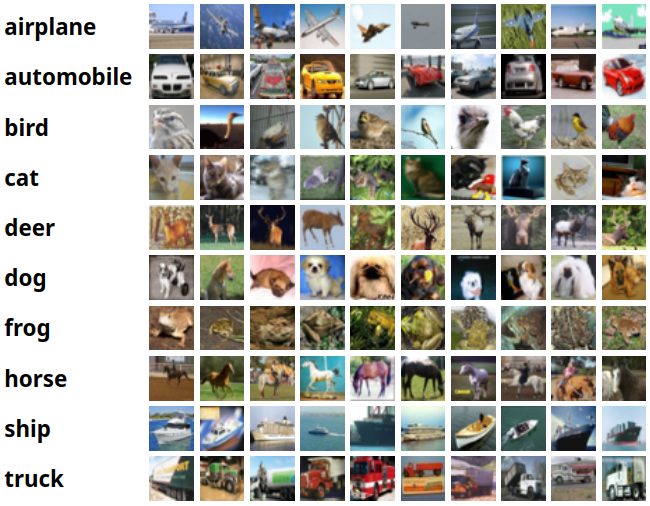
\includegraphics[width=2.5in]{cifar10_example.png}
  \caption{The CIFAR-10 dataset.}
  \label{CIFAR example}
\end{figure}